\section{Scenario Simulation}~\label{sec:task}

\begin{table*}[!htp]
\setlength{\tabcolsep}{2pt}
\centering
\resizebox{\textwidth}{!}{\begin{tabular}{c|c|c|c|c|c|c|c|c|c|c|c}
    \toprule
    \multirow{2}{*}{\textbf{Scenario}}                                          & \multirow{2}{*}{\textbf{Task}}                                                                   & \multirow{2}{*}{\textbf{Paper}}                      & \multicolumn{4}{c|}{\textbf{Environment}}                                   & \multicolumn{3}{c|}{\textbf{Director Role}}                   & \multirow{2}{*}{\textbf{Organization}} & \multirow{2}{*}{\textbf{Communication}} \\ \cline{4-10}
                                                                                &                                                                                                  &                                                      & \textbf{Configuration} & \textbf{State} & \textbf{History} & \textbf{Tools} & \textbf{Planner} & \textbf{Coordinator} & \textbf{Integrator} &                                        &                                         \\ \midrule
    \multirow{29}{*}{\begin{tabular}[c]{@{}c@{}}Dialog- \\ Driven\end{tabular}} & \multirow{5}{*}{\begin{tabular}[c]{@{}c@{}}Social \\ Interaction\end{tabular}}                   & Sotopia~\cite{zhou2023sotopia}                       & \checkmark             & \checkmark     & \checkmark       &                &                  &                      &                     & static,single                          & UNL                                     \\ \cline{3-12} 
                                                                                &                                                                                                  & Elicitron~\cite{ataei2024elicitron}                  & \checkmark             &                & \checkmark       &                &                  &                      &                     & static,multi                           & UNL                                     \\ \cline{3-12}
                                                                                &                                                                                                  & APAM~\cite{yang2024social}                           & \checkmark             &                & \checkmark       &                &                  &                      &                     & static,single                          & UNL                                     \\ \cline{3-12}
                                                                                &                                                                                                  & SimuLife++~\cite{yan2024social}                      & \checkmark             &                & \checkmark       &                &                  &                      &                     & static,single                          & UNL                                     \\ \cline{3-12}
                                                                                &                                                                                                  & Self-Emotion~\cite{zhang2024self}                    & \checkmark             &                & \checkmark       &                &                  & \checkmark           &                     & dynamic,single                         & UNL                                     \\ \cline{2-12}
                                                                                & \multirow{9}{*}{\begin{tabular}[c]{@{}c@{}}Question \\ Answering\end{tabular}}                   & ICL-AIF~\cite{fu2023improving}                       & \checkmark             &                & \checkmark       &                &                  & \checkmark           &                     & static,single                          & UNL                                     \\ \cline{3-12}
                                                                                &                                                                                                  & FORD~\cite{xiong2023examining}                       & \checkmark             &                & \checkmark       &                &                  & \checkmark           &                     & static,multi                           & UNL                                     \\ \cline{3-12}
                                                                                &                                                                                                  & du et al.~\cite{du2023improving}                     & \checkmark             &                & \checkmark       &                &                  &                      &                     & static,single                          & UNL                                     \\ \cline{3-12}
                                                                                &                                                                                                  & MAD~\cite{liang2023encouraging}                      & \checkmark             &                & \checkmark       &                &                  & \checkmark           &                     & static,single                          & UNL                                     \\ \cline{3-12}
                                                                                &                                                                                                  & ChatEval~\cite{chan2023chateval}                     & \checkmark             &                & \checkmark       &                &                  &                      & \checkmark          & static,single                          & UNL                                     \\ \cline{3-12}
                                                                                &                                                                                                  & AutoGen~\cite{wu2023autogen}                         & \checkmark             &                & \checkmark       & \checkmark     &                  &                      &                     & dynamic,single                         & UNL                                     \\ \cline{3-12}
                                                                                &                                                                                                  & AmazonHistoryPrice~\cite{xia2024measuring}           & \checkmark             &                & \checkmark       &                &                  &                      &                     & static,single                          & UNL                                     \\ \cline{3-12}
                                                                                &                                                                                                  & DoG~\cite{ma2024debate}                              & \checkmark             &                & \checkmark       & \checkmark     &                  &                      &                     & dynamic,single                         & UNL                                     \\ \cline{3-12}
                                                                                &                                                                                                  & ChatLLM~\cite{hao2023chatllm}                        & \checkmark             &                &                  &                &                  &                      &                     & static,single                          & UNL                                     \\ \cline{2-12}
                                                                                & \multirow{15}{*}{Game}                                                                           & xu et al.\cite{xu2023exploring}                      & \checkmark             &                & \checkmark       &                &                  &                      &                     & static,multi                           & UNL                                     \\ \cline{3-12}
                                                                                &                                                                                                  & ReCon~\cite{wang2023avalon}                          & \checkmark             &                & \checkmark       &                &                  &                      &                     & static,multi                           & UNL                                     \\ \cline{3-12}
                                                                                &                                                                                                  & MachineSoM~\cite{zhang2023exploring}                 & \checkmark             &                & \checkmark       &                &                  &                      &                     & dynamic,single                         & UNL                                     \\ \cline{3-12}
                                                                                &                                                                                                  & AvalonBench~\cite{light2023text}                     & \checkmark             &                & \checkmark       &                &                  &                      &                     & static,multi                           & UNL                                     \\ \cline{3-12}
                                                                                &                                                                                                  & lan et al.~\cite{lan2023llm}                         & \checkmark             &                & \checkmark       &                &                  &                      &                     & static,multi                           & UNL                                     \\ \cline{3-12}
                                                                                &                                                                                                  & xu et al.~\cite{xu2023language}                      & \checkmark             &                & \checkmark       &                &                  &                      &                     & static,multi                           & UNL                                     \\ \cline{3-12}
                                                                                &                                                                                                  & ThinkThrice~\cite{wu2023deciphering}                 & \checkmark             &                & \checkmark       &                &                  &                      &                     & dynamic,single                         & UNL                                     \\ \cline{3-12}
                                                                                &                                                                                                  & CodeAct~\cite{shi2023cooperation}                    & \checkmark             &                & \checkmark       &                &                  &                      &                     & static,multi                           & UNL                                     \\ \cline{3-12}
                                                                                &                                                                                                  & wu et al.~\cite{wu2024enhance}                       & \checkmark             &                & \checkmark       &                &                  &                      &                     & static,multi                           & UNL                                     \\ \cline{3-12}
                                                                                &                                                                                                  & WWQA~\cite{du2024helmsman}                           & \checkmark             &                & \checkmark       & \checkmark     &                  &                      & \checkmark          & static,multi                           & UNL                                     \\ \cline{3-12}
                                                                                &                                                                                                  & PLAYER~\cite{zhu2024player}                          & \checkmark             &                & \checkmark       &                &                  &                      &                     & dynamic,multi                          & UNL                                     \\ \cline{3-12}
                                                                                &                                                                                                  & GITM~\cite{zhu2023ghost}                             & \checkmark             & \checkmark     & \checkmark       &                & \checkmark       &                      &                     & static,multi                           & UNL                                     \\ \cline{3-12}
                                                                                &                                                                                                  & sreedhar et al.~\cite{sreedhar2024simulating}        & \checkmark             & \checkmark     & \checkmark       &                &                  &                      &                     & static,single                          & UNL                                     \\ \cline{3-12}
                                                                                &                                                                                                  & AmongAgents~\cite{chi2024amongagents}                & \checkmark             & \checkmark     & \checkmark       &                &                  &                      &                     & static,multi                           & UNL                                     \\ \cline{3-12}
                                                                                &                                                                                                  & S-Agents~\cite{chen2024s}                            & \checkmark             & \checkmark     & \checkmark       &                & \checkmark       & \checkmark           &                     & dynamic,single                         & UNL                                     \\ \cline{1-12}
    \multirow{42}{*}{\begin{tabular}[c]{@{}c@{}}Task- \\ Driven\end{tabular}}   & \multirow{16}{*}{\begin{tabular}[c]{@{}c@{}}Foundational \\ and Applied \\ Science\end{tabular}} & VIDS~\cite{hassan2023chatgpt}                        & \checkmark             &                & \checkmark       &                &                  &                      &                     & dynamic,multi                          & UNL                                     \\ \cline{3-12}
                                                                                &                                                                                                  & DR-CoT~\cite{wu2023large}                            & \checkmark             &                & \checkmark       &                &                  &                      &                     & static,single                          & UNL                                     \\ \cline{3-12}
                                                                                &                                                                                                  & ChatGPT Research Group~\cite{zheng2023chatgpt}       & \checkmark             & \checkmark     & \checkmark       &                &                  & \checkmark           &                     & dynamic,multi                          & UNL                                     \\ \cline{3-12}
                                                                                &                                                                                                  & MedAgents~\cite{tang2023medagents}                   & \checkmark             &                & \checkmark       &                &                  &                      & \checkmark          & dynamic,multi                          & UNL,SL                                  \\ \cline{3-12}
                                                                                &                                                                                                  & MARG~\cite{d2024marg}                                & \checkmark             &                & \checkmark       &                &                  & \checkmark           &                     & static,multi                           & UNL                                     \\ \cline{3-12}
                                                                                &                                                                                                  & AI Hospital~\cite{fan2024ai}                         & \checkmark             &                & \checkmark       &                &                  &                      & \checkmark          & static,multi                           & UNL,SL                                  \\ \cline{3-12}
                                                                                &                                                                                                  & REVIEWER2~\cite{gao2024reviewer2}                    & \checkmark             &                &                  &                &                  &                      &                     & static,multi                           & UNL                                     \\ \cline{3-12}
                                                                                &                                                                                                  & CosmoAgent~\cite{jin2024if}                          & \checkmark             &                & \checkmark       &                &                  & \checkmark           &                     & dynamic,single                         & UNL                                     \\ \cline{3-12}
                                                                                &                                                                                                  & FPS~\cite{liu2024skepticism}                         & \checkmark             &                & \checkmark       &                &                  &                      &                     & dynamic,single                         & UNL                                     \\ \cline{3-12}
                                                                                &                                                                                                  & ResearchAgent~\cite{baek2024researchagent}           & \checkmark             &                &                  & \checkmark     &                  &                      &                     & static,multi                           & UNL                                     \\ \cline{3-12}
                                                                                &                                                                                                  & Agent Hospital~\cite{li2024agent}                    & \checkmark             &                & \checkmark       &                &                  &                      &                     & dynamic,multi                          & UNL,SL                                  \\ \cline{3-12}
                                                                                &                                                                                                  & CulturePark~\cite{li2024culturepark}                 & \checkmark             &                & \checkmark       &                &                  & \checkmark           &                     & dynamic,single                         & UNL                                     \\ \cline{3-12}
                                                                                &                                                                                                  & SynthPAI~\cite{yukhymenko2024synthetic}              & \checkmark             &                & \checkmark       &                &                  & \checkmark           &                     & dynamic,single                         & UNL                                     \\ \cline{3-12}
                                                                                &                                                                                                  & DreamFactory~\cite{xie2024dreamfactory}              & \checkmark             &                & \checkmark       &                &                  & \checkmark           &                     & static,multi                           & UNL,SL                                  \\ \cline{3-12}
                                                                                &                                                                                                  & AutoTQA~\cite{zhuautotqa}                            & \checkmark             & \checkmark     & \checkmark       & \checkmark     & \checkmark       &                      &                     & static,multi                           & UNL                                     \\ \cline{3-12}
                                                                                &                                                                                                  & DERA~\cite{nair2023dera}                             & \checkmark             &                & \checkmark       &                &                  &                      &  \checkmark         & static,single                          & UNL                                     \\ \cline{2-12}
                                                                                & \multirow{6}{*}{\begin{tabular}[c]{@{}c@{}}Software \\ Development\end{tabular}}                 & Self-collaboration~\cite{dong2023self}               & \checkmark             &                &                  &                & \checkmark       &                      &                     & dynamic,multi                          & UNL                                     \\ \cline{3-12}
                                                                                &                                                                                                  & ChatDev~\cite{qian2024chatdev}                       & \checkmark             & \checkmark     & \checkmark       & \checkmark     &                  &                      &                     & static,multi                           & UNL,SL                                  \\ \cline{3-12}
                                                                                &                                                                                                  & MetaGPT~\cite{hong2023metagpt}                       & \checkmark             & \checkmark     & \checkmark       & \checkmark     & \checkmark       & \checkmark           &                     & static,multi                           & SL                                      \\ \cline{3-12}
                                                                                &                                                                                                  & Experiential Co-Learning~\cite{qian2023experiential} & \checkmark             & \checkmark     & \checkmark       & \checkmark     &                  &                      &                     & dynamic,multi                          & UNL,SL                                  \\ \cline{3-12}
                                                                                &                                                                                                  & AutoCodeRover~\cite{zhang2024autocoderover}          & \checkmark             &                & \checkmark       & \checkmark     &                  &                      &                     & static,multi                           & UNL,SL                                  \\ \cline{3-12}
                                                                                &                                                                                                  & IER~\cite{qian2024iterative}                         & \checkmark             &                & \checkmark       &                &                  &                      &                     & dynamic,single                         & UNL,SL                                  \\ \cline{2-12}
                                                                                & \multirow{20}{*}{\begin{tabular}[c]{@{}c@{}}Other \\ Industries\end{tabular}}                    & Blind Judgement~\cite{hamilton2023blind}             & \checkmark             &                &                  &                &                  &                      &                     & static,single                          & UNL                                     \\ \cline{3-12}
                                                                                &                                                                                                  & TradingGPT~\cite{li2023tradinggpt}                   & \checkmark             & \checkmark     & \checkmark       &                &                  &                      &                     & dynamic,single                         & UNL                                     \\ \cline{3-12}
                                                                                &                                                                                                  & Information Bazaar~\cite{weissrethinking}            & \checkmark             &                & \checkmark       &                &                  &                      &                     & static,single                          & UNL                                     \\ \cline{3-12}
                                                                                &                                                                                                  & SimuCourt~\cite{he2024simucourt}                     & \checkmark             &                & \checkmark       &                &                  & \checkmark           & \checkmark          & static,multi                           & UNL,SL                                  \\ \cline{3-12}
                                                                                &                                                                                                  & MATHVC~\cite{yue2024mathvc}                          & \checkmark             &                & \checkmark       &                & \checkmark       &                      &                     & static,multi                           & UNL                                     \\ \cline{3-12}
                                                                                &                                                                                                  & baker et al.\cite{baker2024simulating}               & \checkmark             &                & \checkmark       &                &                  &                      &                     & static,multi                           & UNL                                     \\ \cline{3-12}
                                                                                &                                                                                                  & LawLuo~\cite{sun2024lawluo}                          & \checkmark             &                & \checkmark       &                &                  & \checkmark           &                     & dynamic,multi                          & UNL                                     \\ \cline{3-12}
                                                                                &                                                                                                  & MAIC~\cite{yu2024mooc}                               & \checkmark             & \checkmark     & \checkmark       &                &                  & \checkmark           &                     & dynamic,multi                          & UNL                                     \\ \cline{3-12}
                                                                                &                                                                                                  & CAMEL~\cite{li2023camel}                             & \checkmark             &                & \checkmark       &                & \checkmark       &                      &                     & static,single                          & UNL                                     \\ \cline{3-12}
                                                                                &                                                                                                  & SwiftSage~\cite{lin2024swiftsage}                    & \checkmark             & \checkmark     & \checkmark       &                &                  &                      &                     & static,single                          & UNL                                     \\ \cline{3-12}
                                                                                &                                                                                                  & Multi-Agent Collaboration~\cite{talebirad2023multi}  & \checkmark             & \checkmark     & \checkmark       & \checkmark     &                  &                      &                     & dynamic,single                         & UNL                                     \\ \cline{3-12}
                                                                                &                                                                                                  & CoELA~\cite{zhang2023building}                       & \checkmark             & \checkmark     & \checkmark       &                &                  &                      &                     & static,multi                           & UNL                                     \\ \cline{3-12}
                                                                                &                                                                                                  & RoCo~\cite{mandi2024roco}                            & \checkmark             & \checkmark     & \checkmark       &                &                  &                      &                     & static,single                          & UNL                                     \\ \cline{3-12}
                                                                                &                                                                                                  & AgentVerse~\cite{chen2023agentverse}                 & \checkmark             & \checkmark     & \checkmark       & \checkmark     & \checkmark       &                      &                     & dynamic,multi                          & UNL                                     \\ \cline{3-12}
                                                                                &                                                                                                  & Scalable~\cite{chen2024scalable}                     & \checkmark             & \checkmark     & \checkmark       &                & \checkmark       &                      &                     & dynamic,single                         & UNL                                     \\ \cline{3-12}
                                                                                &                                                                                                  & AutoAgents~\cite{chen2023autoagents}                 & \checkmark             &                & \checkmark       & \checkmark     & \checkmark       &                      &                     & dynamic,single                         & UNL                                     \\ \cline{3-12}
                                                                                &                                                                                                  & OpenAgents~\cite{xie2023openagents}                  & \checkmark             & \checkmark     & \checkmark       & \checkmark     &                  &                      &                     & dynamic,single                         & SL                                      \\ \cline{3-12}
                                                                                &                                                                                                  & TWOSOME~\cite{tan2024true}                           & \checkmark             & \checkmark     &                  &                &                  &                      &                     & static,single                          & -                                       \\ \cline{3-12}
                                                                                &                                                                                                  & ReAd~\cite{zhang2024towards}                         & \checkmark             & \checkmark     & \checkmark       &                & \checkmark       &                      &                     & dynamic,single                         & UNL                                     \\ \cline{3-12}
                                                                                &                                                                                                  & MACNET~\cite{qian2024scaling}                        & \checkmark             &                & \checkmark       &                &                  &                      &                     & dynamic,single                         & UNL                                     \\ \bottomrule
    \end{tabular}
}
\caption{A list of representative works of scenario simulation. UNL: unstructured natural language; SL: structured language.}
\label{tab: task_summary}
\end{table*}


In the real world, individuals do not function in isolation. They frequently engage in collaborative efforts to complete tasks within specific scenarios. This raises a crucial question: can LLM-based agents cooperate like humans or even surpass human performance in achieving collective intelligence? To answer this question, researchers simulate the interactions and collaborations of multiple individuals across various scenarios~\cite{qian2023communicative,hong2023metagpt,wu2023autogen}, ranging from everyday conversations to complex professional tasks, to enhance collective intelligence and problem-solving capabilities. A scenario simulation typically starts with designing a multi-agent system that includes constructing the scenario environment, modeling agent roles, and establishing organizational structures and communication protocols to manage interactions among agents.

In this section, we begin discussing the system composition of a scenario simulation with four key aspects in~\S\ref{subsec:sce_sys}. Following this, we summarize several scenarios that have recently attracted the attention of researchers in~\S\ref{subsec:sce_sce}. Finally, we review the methods and metrics commonly used for evaluating scenario simulations in~\S\ref{subsec:sce_eval}. The overall framework is presented in Figure~\ref{fig:fm_task} and representative works are summarized in Table~\ref{tab: task_summary}.

\subsection{System}\label{subsec:sce_sys}

The diversity of scenarios presents challenges in proposing a unified system applicable to scenarios. 
Most of the current systems can be summarized as \textit{``agents organized to play roles in dedicated environments through constrained communications"}.
Based on this general description, we identify four key concepts in scenario simulations: \textbf{environment}, \textbf{role}, \textbf{organization} and \textbf{communication}.


\subsubsection{Environment}

The environment in scenario simulation defines the specific contexts in which agents operate and interact with each other. Just as humans gather information from their surroundings, agents depend on the environment to receive input from various sources. These signals guide the behaviors and strategies of agents within the system. Thus, a comprehensive understanding of the environment paves the way for agents' decision-making and task continuity. We analyze the environment of existing work by focusing on four key aspects: \textit{configuration}, \textit{state}, \textit{history} and \textit{tools}.

\paragraph{Configuration}

The environment configuration provides basic information, especially essential elements necessary for the tasks and goals in the scenario.
The system will initialize agents accordingly so that they interact with clear objectives.
More specifically, an environment configuration may include \textit{events} in the environment and \textit{profiles} of agents.

\textit{{\ul Events}} are represented as a primary focus that needs to be resolved, such as the specific cases brought before the court~\cite{hamilton2023blind,he2024simucourt,sun2024lawluo,baker2024simulating}, and the topics that serve as the basis for multi-agent debates.~\cite{xiong2023examining,du2023improving,liang2023encouraging,chan2023chateval,wu2023autogen,xia2024measuring,ma2024debate}.

\textit{{\ul Profile}} refers to personalized information relevant to the agents specific to the scenario. Different from the basic attributes described in individual simulation, this module encompasses various aspects of the agents' identities, including their interests, goals, and roles~\cite{hong2023metagpt,yukhymenko2024synthetic,zhang2024self}.
Agents can also be configured to have access to external resources, such as related research papers~\cite{baek2024researchagent}, predefined strategies~\cite{zhang2024self} or disease information~\cite{li2024agent}.

\paragraph{State}

Environment states encompass the information provided by the environment during scenario execution (configurations are fixed at the beginning instead).
They directly influence the agents' decision-making and behavior.
According to how agents receive them, states can be further divided into \textit{observation} and \textit{feedback}.

\textit{{\ul Observation}} involves changes in the environment and the current state of surrounding entities. For example, properties and spatial positions~\cite{lin2024swiftsage,tan2024true,chen2024s,chen2024scalable} of other agents are provided to agents to inform real-time decision-making. Moreover, continuously updating agents' physical states are utilized to establish real-time spatial relationships with their environment and neighboring agents~\cite{zhu2023ghost,chen2024scalable,tan2024true,zhang2024towards}.

\textit{{\ul Feedback}} consists of responses received by agents after they perform actions, which guide future strategy adjustments. Some studies~\cite{talebirad2023multi,chen2024s,sreedhar2024simulating} describe how agents’ cognitive states and strategies are modified based on feedback after each interaction, allowing them to simulate human-like adaptability. Meanwhile, feedback on market events or decisions made by others~\cite{li2023tradinggpt,sreedhar2024simulating} and execution results from external tools~\cite{qian2024chatdev,hong2023metagpt,wu2023autogen} are provided, to facilitate strategy adjustment and guide future actions.

\paragraph{History}

As the scenario runs, past states and interactions accumulate into a series of history records.
Agents can leverage them to adapt to new situations and refine strategies, ensuring more coherent and effective task performance in dynamic environments.
We summarize four widely used methods to process and utilize the history, including \textit{direct integration}, \textit{refinement}, \textit{summarization} and \textit{memory mechanisms}.

\textit{{\ul Direct integration}} appends the history to the current input without modification. Agents may retain task continuity by incorporating past dialogue directly into the current session~\cite{du2023improving,liang2023encouraging,wu2023large,wu2023autogen}. Excessive content is truncated to fit token limits while preserving key historical information~\cite{chen2024scalable,xie2023openagents}.

\textit{{\ul Refinement}} iteratively updates and enhances responses based on the history. Ma et al.~\cite{ma2024debate} uses a subgraph-focusing mechanism to refine answers, allowing agents to optimize outcomes after each reasoning step. Similarly, Weiss et al.~\cite{weissrethinking} and D'Arcy et al.~\cite{d2024marg} iteratively improves initial answers to converge to more accurate results.

\textit{{\ul Summarization}} distills essential insights from the history. This can be achieved by synthesizing core actions from multiple plans to establish a reference for diverse scenarios~\cite{zhu2023ghost}, summarizing reports from multiple agents to consolidate findings~\cite{tang2023medagents}, and sharing key solutions subtasks~\cite{qian2024chatdev} to avoid lengthy dialogue histories.

\textit{{\ul Memory mechanisms}} process the history through agents' memory modules. This dynamic approach enables agents to preserve relevant information both within and across sessions \cite{li2023tradinggpt,chen2023autoagents,liu2024skepticism,qian2024iterative,qian2024scaling,xie2024dreamfactory,lin2023agentsims,li2023metaagents}. In addition, Hong et al.~\cite{hong2023metagpt} proposed shared message pools to further enhance communication efficiency, where agents exchange structured messages directly and retrieve information in a personalized manner.

\paragraph{Tools}

External tools offer specialized functionalities related to scenario simulation tasks, enabling more accurate and precise outcomes. The spectrum of tools utilized in scenario simulation encompasses a wide range, from programming languages such as Python and SQL to APIs facilitating external interactions. Generally, Python is mainly employed to execute and verify programmes~\cite{qian2024chatdev,hong2023metagpt,wu2023autogen}. SQL~\cite{zhuautotqa} and knowledge graphs query tools ~\cite{baek2024researchagent,ma2024debate} have been harnessed to retrieve external structured data. In certain scenarios, task-related tools such as calculators, predefined tools, and APIs~\cite{chen2023autoagents,xie2023openagents}  are also utilized to provide intermediate results, simplifying the processing workflow of agents.

\subsubsection{Role}

In scenario simulations, we assign agents distinct roles based on their tasks and functionalities.
As demonstrated in Figure~\ref{fig:fm_task}, there are two groups of roles in a typical setting: \textit{participants} carry out the tasks within the scenario, and \textit{directors} manage the task execution processes while providing necessary assistance.
Each role has its own responsibility that emphasizes different aspects of the system's operations.
They collaborate to achieve the system's overall goals.

\paragraph{Participants} 

Participants are the key members that actively engaged in task execution and discussion.
Their organization and communication are the core of task completion in scenario simulations.
Participants can be further classified into \textit{communicators} and \textit{workers} according to their tasks.

\textit{{\ul Communicators}} primarily focus on communication, such as information exchange, feedback, and task guidance. Specifically, this kind of agents can process information for certain disciplines and research applications~\cite{hamilton2023blind,nair2023dera} and advocate diverse viewpoints~\cite{xiong2023examining,hao2023chatllm}, claims~\cite{liang2023encouraging} and underlying needs~\cite{ataei2024elicitron,li2024culturepark}. 

\textit{{\ul Workers}} are directly involved in task execution and operations, demonstrating specialized skills and efficiency. This typically includes the common professional roles present in each scenario, such as coder and tester in software development~\cite{dong2023self}, buyer and seller in negotiations~\cite{fu2023improving}, doctors and medical professional agents in healthcare domain~\cite{wu2023large,li2024agent}, and receptionist, lawyer, and secretary in the legal contexts~\cite{sun2024lawluo}.


\paragraph{Directors}

While participants execute most of the tasks, directors can provide essential support in crucial aspects such as planning procedures, coordinating communication, and integrating results.
We name them \textit{Planners}, \textit{Coordinators} and \textit{Integrators} respectively.

\textit{{\ul Planners}} play a vital role in task definition and strategic formulation, facilitating effective inter-agent collaboration through tasks such as defining objectives, analyzing user requirements, and optimizing execution plans. Task-specific agents~\cite{li2023camel}, central planners~\cite{chen2023agentverse}, analysts~\cite{dong2023self} and decomposer~\cite{zhu2023ghost} are responsible for breaking down requirements and dividing overarching objectives into specific sub-goals. Product managers~\cite{hong2023metagpt} contribute by creating detailed product requirements documents. Other planners can also refine execution plans according to task requirements~\cite{chen2024scalable}, optimize the process by maximizing the advantage function~\cite{chen2024s} and develop plans based on user inquiries~\cite{zhuautotqa}.

\textit{{\ul Coordinators}} are responsible for managing and coordinating the collaboration between agents to ensure effective task execution, monitor progress, and facilitate cooperation. The project managers~\cite{hong2023metagpt,zheng2023chatgpt} in software development oversee task distribution and project progress, ensuring efficient collaboration among team members throughout the development cycle. Judge assistant agents~\cite{he2024simucourt} aids in organizing information during court proceedings, and the main contact agents~\cite{li2024culturepark} manage intercultural conversations. Additionally, the secretary agents~\cite{jin2024if} manage interactions among civilization agents.
Meanwhile, coordinators also provide feedback to guide better interactions. Critic agents~\cite{fu2023improving} evaluate negotiation strategies and guide agents through iterative learning processes. Judge agents~\cite{xiong2023examining,liang2023encouraging,liang2024debatrix} serve as an authoritative evaluator, assessing arguments and performances during debates.

\textit{{\ul Integrators}} encompass various decision-making and summarization functions critical for guiding the system's trajectory. Deciders~\cite{nair2023dera} autonomously evaluate contributions from the researcher to make informed judgments on the dialogue's outcome. Summarizer agents~\cite{chan2023chateval} enhance communication clarity by providing concise summaries of discussions after each iteration, effectively integrating key points into the ongoing dialogue. In medical scenarios, medical report assistants~\cite{tang2023medagents} compile analyses into a cohesive document that supports collaborative expert discussions, while the medical decision maker ensures that final decisions reflect the collective expertise of the specialists involved. Additionally, the chief physician~\cite{fan2024ai} evaluates diagnostic performance based on accuracy and effectiveness, reinforcing the system's overall reliability. In legal contexts, the judge~\cite{he2024simucourt} oversees judicial processes, making critical decisions grounded in legal arguments and assessing the evidence presented.


\subsubsection{Organization}
Effective task execution necessitates careful coordination and scheduling of the interactions between individual agents. The organizational structures establish how each agent collaborates with others to achieve a goal. Typically, we can depict an organization schema by its \textit{mode} and \textit{structure}.

\paragraph{Mode}
The organizational structure determines whether the relationships among agents remain stable or evolve dynamically throughout the simulation process. In terms of how to organize agents, there are mainly two modes in existing research, i.e., \textit{static} and \textit{dynamic mode}.

\textit{{\ul Static mode}} refers to the organizational structure predefined based on the nature of the tasks. Agents communicate and work in an orderly manner according to these static structures. The static mode can be further divided into single-stage and multi-stage setups. In the single-stage setup, agents follow a fixed structure in multiple rounds of communication, such as structured debates~\cite{nair2023dera,li2023camel,fu2023improving,chan2023chateval}, skill training~\cite{yang2024social,yan2024social} and integrating ideas \cite{hamilton2023blind,hao2023chatllm}. In the multi-stage setup, tasks are divided into distinct stages, and the organization may change with stages. This can be found in the design, coding, and testing stages in software development scenarios following the waterfall model or standardized operating procedures~\cite{qian2024chatdev,hong2023metagpt}, and multi-stage process in judicial scenarios~\cite{he2024simucourt,baker2024simulating} and problem-solving processes~\cite{zhu2023ghost,zhang2023building,ma2024debate}.

\textit{{\ul Dynamic mode}} explores more open and adaptive organizational structures, often relying on dynamic and heuristic communication. This also includes both single-stage and multi-stage setups.  The single-stage setup emphasizes agent collaboration and adaptability in a single stage. The agents can be flexibly created and recruited~\cite{xie2023openagents,chen2023autoagents,ma2024debate,chen2023agentverse,liu2024autonomous}, coordinated through liaison agents~\cite{jin2024if,li2024culturepark}, and self-organized~\cite{chen2024s}. The multi-stage setup mainly features dynamic discussions among agents. Agents can be involved across multiple stages, but they can communicate autonomously based on the current state~\cite{dong2023self,zheng2023chatgpt,tang2023medagents,sun2024lawluo,yu2024mooc}.

\paragraph{Structure} % or Organization Structure
The organization structure, meanwhile, reflects how agents are connected with each other. Typically, an organization can be \textit{layered}, \textit{centralized} or \textit{decentralized}.
\textit{{\ul Layered}} structures adopt a hierarchical framework, with agents assigned to distinct levels. Interactions are predominantly confined to agents within the same level or occur between adjacent layers, thereby facilitating a controlled and organized flow of information\cite{hamilton2023blind,hao2023chatllm,qian2024chatdev}.
\textit{{\ul Centralized}} structures often involve a high-level role (e.g., coordinator) that serves as the core of the organization, overseeing communication and functioning as the central hub for interactions among other agents\cite{jin2024if,li2024culturepark,fan2024ai}.
\textit{{\ul Decentralized}} structures, in contrast, is more flattened, where agents can engage in peer-to-peer interactions as needed\cite{chan2023chateval,ma2024debate,liang2023encouraging}.

\subsubsection{Communication}
The communication between agents controls the transmission of information. To better understand the internal mechanism of communication, we dissect communication from its \textit{format} and \textit{style}.

\paragraph{Format}
From the perspective of information format, there exist two common communication protocols: \textit{unstructured natural language} and \textit{structured language}.

\textit{{\ul Unstructured natural language}} is most commonly used in multi-agent communication, enabling flexible and immediate exchanges through free-form, conversational language that mirrors human dialogue~\cite{nair2023dera,li2023camel,fu2023improving,xiong2023examining,du2023improving,zheng2023chatgpt,yang2024social,yan2024social}. Communication based on natural language is diverse and flexible, but it can also suffer from issues such as ambiguity and redundancy.

\textit{{\ul Structured language}}, such as code and JSON documents, is another protocol that may alleviate the issues from natural language.
In software development, agents transit information between phases through code~\cite{hong2023metagpt,qian2024chatdev}. In the medical domain, structured summaries of reports are utilized to gain key insights~\cite{tang2023medagents}. In addition to predefined formats, agents can also autonomously choose the appropriate format during interactions to improve efficiency~\cite{chen2024beyond,chen2024optima}. Recently, more complex communication protocols using more than one language have been designed to improve communication~\cite{marro2024scalable}.

\paragraph{Style}
Communication, by nature, can be \textit{cooperative} or \textit{competitive} regarding its style.
In \textit{{\ul cooperative}} communication, agents share a common objective, aiming to optimize collective outcomes, like software development\cite{dong2023self,qian2024chatdev,hong2023metagpt}, medical diagnosis\cite{tang2023medagents,fan2024ai}, and case handling\cite{hamilton2023blind,sun2024lawluo}.
In contrast, agents in \textit{{\ul competitive}} communication typically hold differing viewpoints and positions, each striving to achieve individual objectives. Such scenarios are commonly found in settings like games\cite{xu2023exploring,du2024helmsman,wang2023avalon} and debates\cite{xiong2023examining,liang2023encouraging,fu2023improving}, where agents maintain opposing stances and seek to outmaneuver each other.

\subsection{Scenario}\label{subsec:sce_sce}
Using the collective capabilities of agents with specialized expertise, scenario simulations have been applied to various domains. Here we divide different scenarios into two groups: \textbf{dialog-driven} ones that cover social interaction and question-answering, and \textbf{task-driven} ones that focus on specialized tasks.

\subsubsection{Dialog-Driven Scenario}
Dialog-driven scenarios encompass scenarios in people's daily lives where the dialog itself is centered, such as those for social or entertainment purposes.
These scenarios share a common emphasis on tackling general goals that are not related to any specific task or domain.
We identify three primary types of dialog-driven scenarios: \textit{social interaction}, \textit{question-answering}, and \textit{game} scenarios.


\paragraph{Social Interaction}
Some works focus on task completion in simple social interaction scenarios, typically involving social tasks between two or a few agents, such as persuasion or comforting a partner. Zhou et al.~\cite{zhou2023sotopia} discusses the social intelligence of agents in social scenarios, revealing significant performance differences among models across different dimensions. The exploration in social intelligence is further extended to objective action-level evaluation~\cite{wang2024towards} and diverse scenarios and others' information reasoning\cite{mou2024agentsense}. Furthermore, some works propose interactive learning methods~\cite{yang2024social,wang2024sotopia,zhou2024real} to help learn social skills.

\paragraph{Question Answering}
Another mainstream scenario is the question answering, emphasizing collaborative processes, strategic reasoning, and integration to enhance model performance. On the one hand, some studies focus on improving reasoning through debate. FORD~\cite{xiong2023examining} facilitates a three-stage commonsense reasoning debate, demonstrating that LLMs can reach consensus even amidst inconsistencies. MAD~\cite{du2023improving}, involves agents debating under a judge's supervision, addressing the Degeneration-of-Thought problem. In addition, a ``society of minds" approach~\cite{du2023improving} is presented to guide multiple debate rounds, improving mathematical reasoning and factual accuracy while reducing hallucinations. On the other hand, some works focus on optimizing strategies in strategic reasoning and negotiation. OG-Narrator~\cite{xia2024measuring} is proposed to improve negotiation strategies, increasing the Buyers' deal success rates. Ma et al.~\cite{ma2024debate} utilize a subgraph-focusing mechanism and a multi-role debate team to improve reasoning accuracy and reliability, outperforming existing methods.

\paragraph{Game}
Games provide a unique platform for exploring scenario simulation, evolving from basic game reproduction to complex social dynamics.
Early studies, such as \cite{xu2023exploring,wang2023avalon}, introduce Werewolf and Avalon to examine LLM performance in communication games, specifically investigating how LLMs handle aspects like trust and leadership. 
Building on these complex interactions, reinforcement learning frameworks in \cite{xu2023language,wu2024enhance} allow agents to adapt their strategies, achieving near-human-level decision-making.
To explore deeper social phenomena, \cite{wu2024enhance,zhu2024player} expand on game dynamics by incorporating tools that enhance memory, reasoning, and adaptability. 
Additionally, \cite{du2024helmsman} examines the role of opinion leadership, while \cite{wu2023deciphering,shi2023cooperation,gong2023mindagent} tackle ad hoc teamwork, where agents adapt and collaborate without predefined protocols, revealing both the challenges and potential of LLM agents in team-based collaboration.

\subsubsection{Task-Driven Scenario}
In task-driven scenarios, agents role-play personas with specific functions for a certain task or task-set.
Most of these scenarios fall into one or more specific domains related to the tasks.
Here, agents are increasingly leveraged to solve complex, domain-specific problems by automating tasks and improving decision-making processes.

\paragraph{Foundational and Applied Science}
Science domains, such as medicine, mathematics, data science, and content analysis, have been popular experimental fields for scenario simulation. In the medical domain, medical reasoning and automating diagnostic processes have been refined through innovative methodologies such as chain-of-thought prompting and multi-agent collaboration\cite{wu2023large,tang2023medagents,li2024agent,bao2024piors}.
Zheng et al.\cite{zheng2023chatgpt} integrates ChatGPT with Bayesian optimization techniques to enhance research workflows in chemistry laboratories, demonstrating significant improvements in efficiency and productivity. Hassan et al.\cite{hassan2023chatgpt} introduce a conversational framework that enables seamless interaction with machine learning models, specifically for tasks like data visualization and predictive analytics. These studies demonstrate the potential of LLM-based agents to transform traditional research patterns.

\paragraph{Software Development}
Recent research has increasingly focused on harnessing agents to address complex challenges in software development and life-cycle management. Early works focus on designing frameworks for collaborative code generation. Dong et al.~\cite{dong2023self} presents a self-collaboration framework where LLM agents function as distinct ``experts," each managing specific subtasks to facilitate autonomous collaborative code generation. Building on this, ChatDev\cite{qian2024chatdev}, a chat-powered framework utilizes unified language-based communication among agents to effectively address design, coding, and testing phases. Meanwhile, Hong et al.~\cite{hong2023metagpt} enhances LLM collaborations by encoding Standardized Operating Procedures into prompts, enabling agents to verify results and produce coherent solutions through an assembly line approach. Afterward, some works focus on enabling agents to learn from past experiences and refine their processes over time
~\cite{qian2023experiential,qian2024iterative}. Further efforts focus on autonomous issue resolution and program understanding~\cite{zhang2024autocoderover}. These studies show the potential of multi-agent collaboration in software engineering, offering robust tools for automatic development and management.


\paragraph{Other Industries}
In the realm of broad social science, several studies leverage multi-agent systems to enhance decision-making processes across diverse fields, such as journalism~\cite{liu2024aipress}, judiciary, economics, and education. In the judicial field, legal consultations have been improved through LawLuo~\cite{sun2024lawluo}, which simulates collaborative discussions. Hamilton et al.~\cite{hamilton2023blind} and He et al.~\cite{he2024simucourt} design multi-agent systems to simulate U.S. Supreme Court decisions and court trials through detailed steps such as debate, resource retrieval, and decision refinement, complemented by additional benchmarks that enhance legal article generation. In the economic sector, Li et al.~\cite{li2023tradinggpt} propose a multi-agent framework with layered memory to improve LLM performance in stock trading. Additionally, Weiss et al.~\cite{weissrethinking} address the buyer's inspection paradox in information markets by simulating a marketplace where intelligent agents use LLMs to navigate information access and biases, exploring the impact of pricing and budgets on outcomes. In the education domain, MAIC~\cite{yu2024mooc}, a system simulating AI-enhanced classrooms has contributed to the development of a comprehensive AI-driven online education platform. Yue et al.~\cite{yue2024mathvc} presents MATHVC, an LLM-driven virtual classroom designed to simulate interactions among students, thereby fostering the development of mathematical skills.

\begin{figure*}[!t]
    \centering
    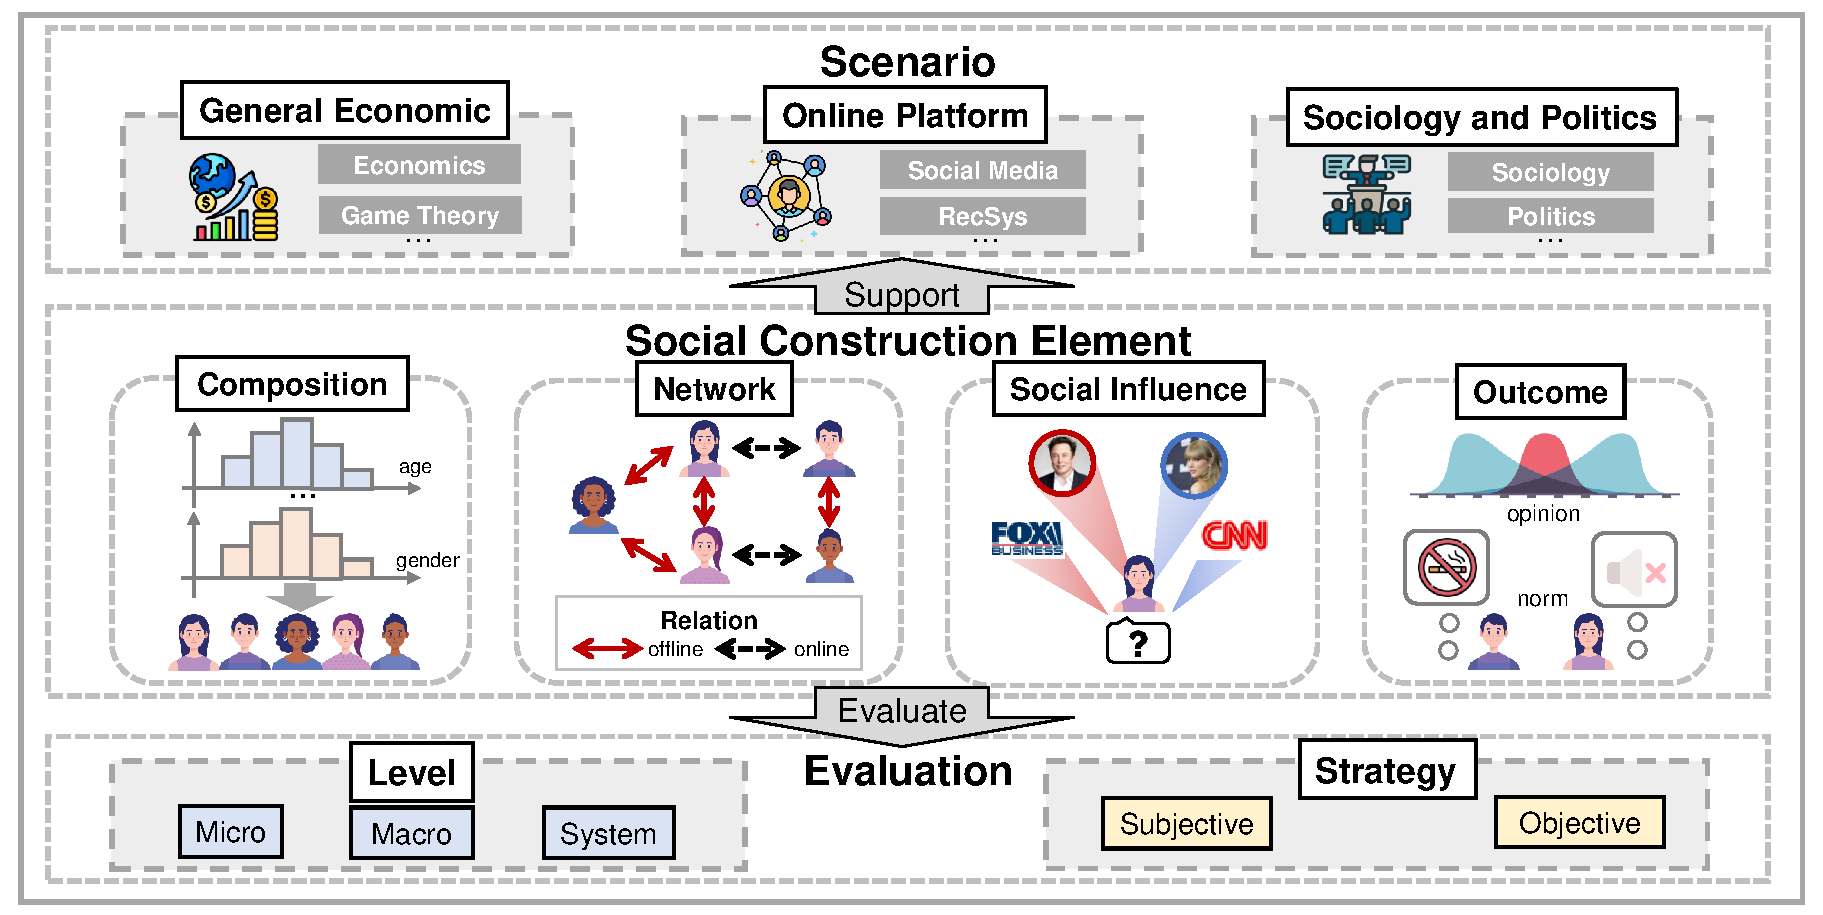
\includegraphics[width=\linewidth]{figs/fm_soc_v2_2.pdf}
    \caption{Illustration of society simulations. To construct society simulations, the corresponding society's {\ul construction elements}, i.e., composition, network, social influence and outcomes need to be carefully designed. Building on this, various {\ul scenarios} can be simulated. The performance of individuals and the overall performance of the system are {\ul evaluated}.}
    \label{fig:fm_soc}
\end{figure*}


\subsection{Evaluation}\label{subsec:sce_eval}
For scenario simulations, the evaluation focuses on how well the tasks of the scenarios are solved. Based on the scope of the evaluation, it can be categorized into \textbf{task evaluation}, \textbf{sub-task evaluation} and \textbf{system evaluation}, each employing various \textit{{automatic}}, \textit{{LLM-based}}, and \textit{{human}} evaluation methods to assess performance.

\paragraph{Task Evaluation}
Task Evaluation measures the overall performance of tasks assigned to the scenario. The evaluation can carried out in automatic ways or by LLMs or humans. In terms of \textit{{\ul automatic}} evaluation, predefined metrics and mathematical tools are used to objectively assess the task outcomes, such as accuracy~\cite{hamilton2023blind,xiong2023examining}, pass@k~\cite{li2023camel} for coding tasks, success rate, and coverage for exploration~\cite{zhu2023ghost}, and deal price for negotiation~\cite{fu2023improving}. These methods are efficient and scalable but may overlook complex behaviors. Thus, \textit{{\ul LLMs}}~\cite{hao2023chatllm} and \textit{{\ul human }}experts~\cite{li2023camel,liang2023encouraging} have been applied to provide more nuanced evaluation for qualitative tasks and compare solutions based on specific criteria.

\paragraph{Sub-Task Evaluation}
Sub-task Evaluation assesses the completion of sub-tasks within a scenario simulation and their impact on overall task performance. It serves as a process evaluation for the execution of complex tasks. The \textit{{\ul automatic}} evaluation uses metrics like transport rate, average steps, task success rate, re-plan attempts, and efficiency improvement to assess sub-task performance and strategy efficiency~\cite{zhang2023building,mandi2024roco}. Completeness, executability, and consistency metrics are often applied in software generation tasks~\cite{qian2024chatdev,qian2023experiential}. \textit{{\ul LLM-based}} evaluation focuses on pairwise comparisons or win rate judgments, capturing qualitative aspects of sub-task performance~\cite{qian2024chatdev}. Meanwhile, \textit{{\ul human}} evaluation relies on participants to provide subjective assessments on metrics such as executability, revision costs, or comment quality, offering practical insights into sub-task performance~\cite{hong2023metagpt,d2024marg}.


\paragraph{System Evaluation}
System Evaluation aims to capture the effectiveness and efficiency of the system in a scenario simulation as a whole. \textit{{\ul Automatic}} evaluation relies on metrics such as token consumption, task success rate, and human-likeness scores to measure the efficiency and realism of agents~\cite{tan2024true}. Additional metrics like accuracy, precision, recall, and F1 scores are used to assess system accuracy and consistency in diagnostic or predictive tasks~\cite{fan2024ai}. \textit{{\ul LLM-based}} evaluation often involves GPT-4 to assess qualitative aspects, such as human-likeness or diagnostic report quality~\cite{tan2024true,li2024agent}. \textit{{\ul Human}} evaluation typically involves subjective assessments, such as rating instructional content for tone, clarity, and supportiveness on a Likert scale~\cite{yu2024mooc}, often used to complement automatic methods and capture human perspectives on system outputs.


